\renewcommand{\thechapter}{4}

\chapter{Optical speckle, a Gaussian beam model}\label{speckle_chapter}
An optical speckle is a  powerful tool for creating disordered potentials for atomic systems\cite{billy2008direct,kondov2011three}.  It was studied in the 1970s \cite{goodman2007speckle}, the strength of the resultant potential is under direct experimental control: the spatial correlation length is tunable and the correlation function is well known. 

Optical speckle can be understood as the self-interfering wave field of a laser after acquiring a random phase by reflection off rough surfaces or transmission through disordered media, called a diffuser~\cite{goodman2007speckle}. We will focus on the transmission case and assume that the spatial scale of the disorder $\sigma$ is small in comparison to the laser beam size and that the diffuser transmits light uniformly. The transmitted field can be intuitively thought of as of many waves scattered from microscopic elements comprising the diffuser.  So randomness arises.  As a disordered field, optical speckle is characterized by its intensity distribution, spatial intensity correlation function, and power spectral density (PSD).  

As shown in Fig.~\ref{fig:speckle1} shows, ray optics in the paraxial limit provides a simple and useful approach to estimating the on-axis beam properties of a speckle beam a distance $z$ beyond a diffuser.  As a collimated laser beam of wavelength $\lambda$ travels through a diffuser of diameter $D_d$, it acquires a local divergence angle $\theta_d\simeq \lambda / (2 \sigma)$.   

Fig.~\ref{fig:speckle1}(a) depicts the simplest case consisting of an isolated diffuser, for which there are two qualitatively different regimes: A near-field regime with $z < D_d / (2 \theta_d)$, where the typical length scale of optical speckle is $\sigma$, and a far-field regime where the numerical aperture (NA) of the diffuser increases the speckle scale to $(\lambda / 2)\times(2 z /D_d )$.  This simple approach is insufficient because we are interested in micrometer scale speckle, which is far smaller than the 10 to 100 micrometer scale of $\sigma$ for commercial diffusers.

In Fig.~\ref{fig:speckle1}(b) we add a lens with diameter $D_L$ and focal length $f$ just after the diffuser.  In the focal plane of the lens, the speckle scale is set by the lens NA, giving a speckle length scale $\lambda f / D_L$, independent of $\sigma$. In contrast, the beam width at the focal plane $w(f) \simeq 2 f \theta_d$ is set by the speckle scale $\sigma$ and not the lens diameter.

In this chapter, we will derive the origin of these design guidelines from the paraxial wave equation.
\begin{figure}[htbp]
    \centering
    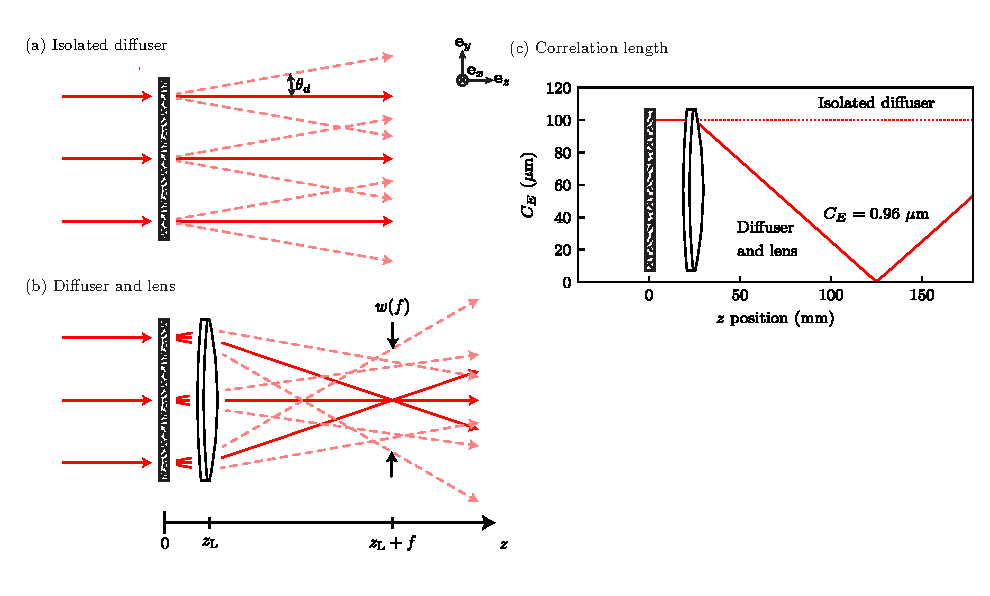
\includegraphics[width=\textwidth]{Chapter4_secs/speckle1.pdf}
    \caption{Optical speckle schematic. (a) A collimated beam is transmitted through a rough medium and its intensity is measured in plane $z$. (b) The diverged beam after the rough medium is imaged by a lens at plane $z=z_L$ and $f$ is the focal point of the lens. (c) Field-field correlation length for a Gaussian speckle beam initially with $\sigma=100\ \mu{\rm m}$ and $w=25\ {\rm mm}$ as a function of propagation distance. The red curves plot $c_E(z)$ computed with (solid) and without (dashed) a lens with focal length $f=100\ {\rm mm}$ at $z_L=25\ {\rm mm}$. }
    \label{fig:speckle1}
\end{figure}

\section{Gaussian beam equations with speckle}
We focus on monochromatic optical electric fields $E({\bf x}, t)$ with angular frequency $\omega$ traveling predominantly along ${\bf e}_z$.  Such waves can be decomposed as $E({\bf x}, t) = E_\perp({\bf r}; z) \exp[i(k_0 z -\omega t)]$, where $E_\perp({\bf r}; z)$ describes the transverse structure of the electric field with the high spatial frequencies associated with the nominal propagation along ${\bf e}_z$ factored out.  For spatial scales in excess of the optical wavelength the transverse field obeys the paraxial wave equation
\begin{equation}\label{para equation}
    -2i k_0 \partial_z E_\perp({\bf r}; z) = \left[-\nabla_\perp^2 + k_0^2 \chi({\bf r}; z)\right] E_\perp({\bf r}; z)
\end{equation}
traveling in a material with relative susceptibility $\chi({\bf r}; z)$.  We will suppress the $\perp$ subscript in the remainder of our discussion.

Upon traversing through a thin but disordered material with susceptibility $\chi({\bf r}) $ and thickness $\delta z$, an initially Gaussian wave field $E^-({\bf r}, 0) = E_0\exp{-{\bf r}^2/w^2}$ acquires a position dependent complex phase $\phi({\bf r}) = \chi({\bf r}) k_0 \delta z/2$.  The resultant field
\begin{equation}
    E^+({\bf r}, 0) = E^-({\bf r}, 0)\exp[- i \phi({\bf r})]
\end{equation}
carries the imprint of the disordered medium. The field a distance $z$ beyond the speckle plate follows from
\begin{align}\label{para field}
    E({\bf r}; z) &= \frac{-i k_0}{2\pi z}\int d^2{\bf r'} E^+({\bf r'}; 0) e^{-i k_0|{\bf r}-{\bf r'}|^2/2z},
\end{align} 
the formal solution to the paraxial wave equation Eq.~(\ref{para equation}).  We model typical diffusion plates, for which: (1) the correlation function of the susceptibility $\langle \chi({\bf r_1})\chi({\bf r_2}) \rangle$ depends only on relative distance $|{\bf r_1}-{\bf r_2}|$, where $\langle ... \rangle$ denotes the ensemble average over disorder realizations. (2) the variation of the imprinted phase $\phi({\bf r})$ is much larger than $2\pi$ with
\begin{align}\label{eq:zeromean}
\langle \exp\left[- i \phi({\bf r}_1)\right]\rangle &= 0,
\end{align} 
i.e., $\phi({\bf r})$ is uniformly distributed over the interval $[-\pi,\pi]$.
 
We turn to the field-field correlation function
\begin{equation}\label{C_E}
\begin{aligned}
    C_E({\bf r}_1,{\bf r}_2;z) &=\langle E({\bf r}_1; z)E^\ast({\bf r}_2; z)\rangle\! -\! \langle E({\bf r}_1; z)\rangle\langle E^\ast({\bf r}_2; z)\rangle
\end{aligned}
\end{equation}
to characterize the statistical properties of the disordered electric field.  Eq.~\eqref{eq:zeromean} implies that the second term is zero.  At $z=0$, the uniform phase distribution implies $\langle E^+({\bf r}; 0) \rangle = 0$, giving
\begin{align*}
\frac{C_E({\bf r}_1,{\bf r}_2;0)}{E_0^2 } &= \exp\left(-\frac{{\bf r}_1^2 + {\bf r}_2^2}{w^2}\right) \langle \exp\left\{- i \left[\phi({\bf r}_1)-\phi({\bf r}_2)\right]\right\}\rangle.
\end{align*}
Under the assumptions of the typical diffusion plates, we model the phase-phase correlation function 
\begin{align}\label{gaussian C_E}
\langle \exp\left\{- i \left[\phi({\bf r}_1)-\phi({\bf r}_2)\right]\right\}\rangle &= \exp(-\frac{|{\bf r}_1-{\bf r}_2|^2}{\sigma^2}), 
\end{align} 
with a Gaussian decay of width $\sigma$ that is amenable to the following analytic treatments.  The relation
\begin{align}\label{eq:sum_CE_zero}
\langle \exp\left\{- i \left[\phi({\bf r}_1)+\phi({\bf r}_2)\right]\right\}\rangle &= 0, 
\end{align} 
that follows from Eq.~\eqref{eq:zeromean}, in conjunction with the assumption that the correlation function depends only on relative distance, will be useful as well.

We first consider the case illustrated by Fig.~\ref{fig:speckle1}(a) where a Gaussian beam goes through a large disordered medium. The field-field correlation function at all positions following the disordered medium  can be exactly computed and takes the form 
\begin{align}
\frac{C_E({\bf r}_1,{\bf r}_2;z)}{E_0^2} =& \left[\frac{w}{w(z)}\right]^2 \exp(-ik_0\frac{{\bf r}_1^2 - {\bf r}_2^2}{2 R(z)})\label{eq:C_E}\\
&\times \exp(-\frac{{\bf r}_1^2 + {\bf r}_2^2}{w(z)^2})\exp(-\frac{|{\bf r}_1-{\bf r}_2|^2}{\sigma(z)^2}) \nonumber 
\end{align}
reminiscent of that of Gaussian beams.

This correlation function is characterized in terms of three $z$-dependent functions: the beam waist $w(z)$, the radius of curvature $R(z)$, and the correlation length $\sigma(z)$.  Each of these is simply related to a reduced Rayleigh range $z_{\rm R}^* = z_{\rm R}/M$, with conventional Rayleigh range $z_{\rm R} = k_0 w^2/2$ and beam quality factor $M^2 = 1+2w^2/\sigma^2$.  The resulting coefficients
\begin{align}
    \left[\frac{w(z)}{w}\right]^2 &= \left[\frac{\sigma(z)}{\sigma}\right]^2 = 1+\left(\frac{z-z_0}{z_{\rm R}^*}\right)^2\label{eq:rayleigh}
\end{align}
and
\begin{align}
    \frac{R(z)}{z-z_0} = 1 +\left(\frac{z_{\rm R}^*}{z-z_0}\right)^2
\end{align}
take the same form as a usual Gaussian beam focused at $z_0$.  Lastly, as in Fig.~\ref{fig:speckle1}(b), an ideal lens with focal length $f$ at position $z_L$ gives new Gaussian beam parameters defined by
\begin{align}\label{lens making}
\frac{w^\prime}{w} &= \frac{\sigma^\prime}{\sigma} = f \left[\left(z_0'-z_L-f\right)^2+z_{\rm R}^{*2}\right]^{-1/2}
\end{align}
and
\begin{align*}
\left(z_0^\prime-z_L\right)^{-1} &=  f^{-1} - \left[\left(z_L-z_0\right) + \frac{z_{\rm R}^{*2}}{z_L-z_0-f} \right]^{-1}
\end{align*}

where the first expression defines the magnification and the second is analogous to the usual lens makers equation~\cite{Self1983}.  While this leaves $M^2$ unchanged, the Rayleigh range is altered owing to the change in $w$.  All together these relations fully define field-field correlation function $C_E$ throughout an ideal imaging system. 

In most quantum-gas experiments, optical potentials are created using laser light in the far detuned limit, thereby experiencing a potential proportional to the optical intensity
\begin{equation}\label{intensity}
    I({\bf r}; z) = \frac{c \epsilon_0}{2} \left|E({\bf r}; z)\right|^2
\end{equation}
not the electric field directly.  The ensemble-averaged intensity 
\begin{align}
\langle I({\bf r}; z) \rangle &= \frac{c \epsilon_0}{2} C_E({\bf r},{\bf r}; z), \label{eq:intensity}
\end{align}
simply related to the field-field correlation function in Eq.~(\ref{eq:C_E}), contains no information about the optical speckle except for the changed $M^2$.

As discussed in the next section, the power spectral density (PSD) of the intensity
\begin{align}
    \rho({\bf k}; z) &= \langle \tilde{I}({\bf k};z)\tilde{I}^*({\bf k};z)\rangle\nonumber \\
    &=  \frac{\pi^2w^2(z)}{4M^2}\exp{-\frac{{\bf k}^2w^2(z)}{4M^2}},\label{psd}
\end{align}
computed using Eq.~\eqref{eq:C_E}, describes the momentum-change imparted by the speckle potential to a moving atomic wavepacket.
\section{Correlation length}
The field-field correlation length
\begin{align}
    c_E(z)^2 &= \frac{\iint |C_E({\bf r}_1,{\bf r}_2; z)||{\bf r}_1-{\bf r}_2|^2d^2{\bf r}_1d^2{\bf r}_2}{\iint |C_E({\bf r}_1,{\bf r}_2; z)|d^2{\bf r}_1d^2{\bf r}_2}\\
    &= \frac{2 w(z)^2 \sigma(z)^2}{2w(z)^2 + \sigma(z)^2} \approx \sigma(z)^2
\end{align}
obtained from Eq.~(\ref{eq:C_E}), sets the scale over which the electric field retains its spatial coherence.  The field-field correlation length is minimized at $z=z_0$, and is always larger than $\sigma$.  Generally, speckle beams operate in the regime $w \gg \sigma$, where there are many speckle grains within a large beam, giving the final approximate relation. 

As was already noted in our ray-optics discussion, this has important implications for experiment design.  For cold atom experiments such as ours, the large momentum-change imparted by short-length scale speckle is essential, where a correlation length at or below the micron scale is desirable.  Since the correlation length available for typical commercial diffusers ranges from $10\ {\rm \mu m}$ to $100\ {\rm \mu m}$, an additional focusing stage is required.  

A focusing lens can easily take the $10\ {\rm \mu m}$ to $100\ {\rm \mu m}$ correlation length available for typical commercial diffusers and create a beam with sub-micrometer correlation length at its focus.  Fig.~\ref{fig:speckle1}(c) compares the correlation length of a beam with (red solid) and without (red dashed) a focusing lens for the specific case of an initial laser beam of wavelength $\lambda = 532\ {\rm nm}$ with Gaussian beam parameters: focal point $z_0=0$, beam waist $w = 25\ {\rm mm}$ and correlation length $\sigma = 100\ \mu{\rm m}$.  This beam is focused by a lens of focal length $f=100\ {\rm mm}$, the correlation length at the focus is $c_E=0.96\ \mu{\rm m}$.  The remaining derived beam parameters are
$M^2 \approx 1.25\times10^5$, $z_R \approx 3.7\ {\rm km}$, and $z_R^* \approx 10.4\ {\rm m}$. 

In \cite{yura1999three}, the space–time evolution of three-dimensional (3D) optical speckle is studied using the ABCD ray-matrix techniques. The optical speckle they studied results from a diffuse object that is illuminated by a Gaussian-shaped laser beam. The field-field correlation length obtained from this approach agrees with our results. In addition, the intensity-intensity correlation length in $z$ direction is calculated in \cite{yura1999three}. In the case the optical speckle is focused by a lens with focal length $f$, the on-axis intensity-intensity correlation length in $z$ direction $L_z$ is of the order of the depth of focus $4f^2/kw^2$. Using the parameters in Fig.~\ref{fig:speckle1}(c), in the focal plane, $L_z \approx 5.4~{\rm \mu m}$. In the free propagation case, $L_z$ grows as $4z^2/kw^2$, and $L_z \gg c_E(z)$ in the far field where $z \gg w$.

\section{Impact of apertures}
In the case of focusing optical speckle as shown in Fig.~\ref{fig:speckle1}(b), a lens of focal length $f$ and diameter $D_L \ll w$ is placed at $z=z_L \leq k_0\sigma^2$. The field in the plane $z=z_L$ before the lens, $E^-({\bf r};z_L)$ is essentially unchanged from field $E^+({\bf r};0)$. The field $E^-({\bf r};z_L)$ passes through the lens aperture, where it acquires a position dependent phase and is truncated outside the lens. The emerging field $E^+({\bf r};z_L)$ propagates to the focal plane $z=f+z_L$ where it is 
\begin{equation}\label{field in z}
    E_f({\bf r}) = \frac{-i k_0}{2\pi f}e^{-i k_0{\bf r}^2/2f}\int \displaylimits_{|{\bf r'}|<\frac{D_L}{2}} d^2{\bf r'} E^+({\bf r'}; 0) e^{i k_0{\bf r}\cdot{\bf r'}/f}.
\end{equation}
When $\sigma \ll D_L \ll w$, the field-field correlation function at the focal plane is
\begin{align}
C_{E,f}({\bf r}_1,{\bf r}_2) \approx & C_0\exp[-\frac{ik_0({\bf r}_1^2-{\bf r}_2^2)}{2f}]\\
&\times\exp[\frac{-k_0^2\sigma^2({\bf r}_1 + {\bf r}_2)^2}{16f^2}]\frac{J_1(k_c \Delta r/2)}{k_c\Delta r /2}.\nonumber
\end{align}
Here $C_0 =  k_0^2E_0^2D_L^2\sigma^2 / 8f^2$ is the peak correlation amplitude; $\Delta r = |{\bf r}_1-{\bf r}_2|$ is the relative position coordinate; and $J_1$ is a Bessel function of the first kind.  The ratio 
\begin{align}
k_c &= k_0\frac{D_L}{f}\label{kc}
\end{align}
is a cutoff above which the PSD of the intensity
\begin{align}
    \rho_f(k) = C_0^2 \frac{2}{\pi k_c^2}\left[ \cos^{-1}\left(\frac{k}{k_c}\right)
     -\frac{k}{k_c}\sqrt{1-\frac{k^2}{k_c^2}}\right]\label{psd_image}
\end{align}
is strictly zero.  Eq.~\eqref{psd_image} is valid near the optical axis where $|{\bf r}_1|,|{\bf r}_2| \ll w(z)$.
\section{Field and intensity probability distribution}\label{prob sec}
In the previous sections, we focused on the average properties of speckle fields.  Here we extend this discussion to predict the probability distribution of electric field strength $P(E)$ and intensity $P(I)$.  Our approach focuses first on $P(E)$, and consists of two steps: (1) we find the regime when the central limit theorem applies, thereby assuring a Gaussian probability distribution; (2) we identify $\langle E \rangle$ and $\langle E^2 \rangle$ as the lowest moments of the distribution, fully defining the Gaussian distribution.

We now interpret the electric field
\begin{align*}
    E({\bf r}; z) &= \frac{-i k_0}{2\pi z}\int d^2{\bf r'} E^-({\bf r}')e^{-i \phi({\bf r'}) } e^{-k_0|{\bf r}-{\bf r'}|^2/2z},
\end{align*} 
of Eq.~\eqref{para field} as a random variable constructed from a sum over incoherent complex phasors.  The cross correlation function (CCF) $\langle E({\bf r}_1; z) E({\bf r}_2; 0)\rangle$ specifies the range over which the initial random field contributes to the final field.  The closed form expression for this CCF is similar to the field-field correlation function in Eq.~\eqref{eq:C_E}; the length scale for the decay of correlations $\sigma_{\rm CCF}(z)$ again obeys  Eq.~\eqref{eq:rayleigh}, but with $M_{\rm CCF}^2=(1 + w^2/\sigma^2 )^2$.  When $w\gg\sigma$, i.e., the initial waist is much larger than the speckle size,  the resulting Rayleigh range reduces to $z_{\rm R, CCF} = k_0 \sigma^2/2$: as if each random source was an individual Gaussian beam with extent $\sigma$.  The criterion that a field $E({\bf r}; z)$ have contributions from many incoherence sources is therefore $\sigma_{\rm CCF}(z)/\sigma\gg1$, i.e., $z\gg z_{\rm R, CCF}$.  

This identifies the central limit theorem's regime of applicability, and we now consider $E({\bf r}; z)$ as a complex valued Gaussian random variable.  The probability distribution for electric field is therefore a function of two independent degrees of freedom, here we select the quadrature variables $E$ and $E^*$, giving $P(E, E^*)$.   Most moments of this quantity are easy to identify using Eqs.~\eqref{para field}, \eqref{eq:zeromean}, \eqref{gaussian C_E} and \eqref{eq:sum_CE_zero}: $\langle E \rangle = \langle E^2 \rangle = 0$, and similarly for $E^*$.   Then Eqs.~\eqref{C_E} and the following discussion assure us that  $\langle E E^* \rangle = \langle |E|^2 \rangle$ takes on a non-zero value.  Together these fully define the Gaussian probability distribution for electric fields
\begin{align}
    P(E, E^*) &= \frac{1}{\pi \langle |E|^2 \rangle} \exp\left(-\frac{|E|^2}{\langle |E|^2 \rangle}\right)\label{eq:dist_fields},
\end{align}
and using Eq.~\eqref{eq:intensity}, the intensity distribution
\begin{align}
    P(I) &= \frac{1}{\langle I \rangle} \exp\left(-\frac{I}{\langle I \rangle}\right) \label{P of int}
\end{align}
follows directly.  The intensity of a speckle field obeys an exponential distribution and the mean of speckle intensity $\langle I \rangle$ should be equal to its standard deviation $\sqrt{\langle I^2 \rangle}$.
\section{Simulated speckle and the comparison to experiment}

\begin{figure}[tbp]
    \begin{center}
    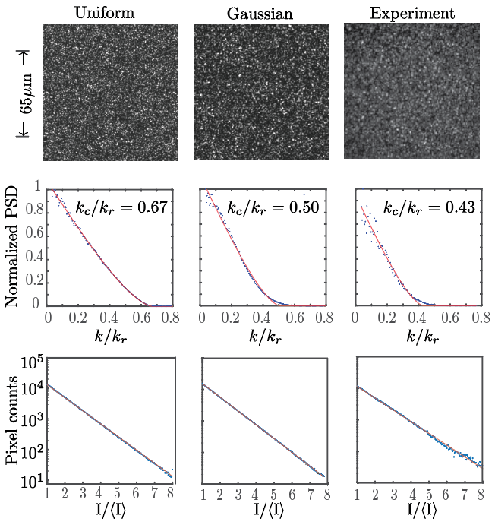
\includegraphics{Chapter4_secs/optical_speckle.pdf}
    \end{center}
    
    \caption{Simulated and measured optical speckle. The columns in the figure correspond to: simulated speckle with uniform laser beam,  simulated speckle from a Gaussian laser beam and measured speckle. In each column, the first row shows the intensity of the optical speckle field. The second row shows the PSD of the intensity shown in the first row (symbols).  The red curve shows a fit of Eq.~(\ref{psd_image}) to the data, along with the resulting $k_c$. The third row histograms the  intensity from the first row. }
    \label{fig:Optical speckle}
\end{figure}

Having now fully set the stage for understanding and creating speckle laser beams, we turn to laboratory confirmation of key prediction of these models relevant to cold atom experiment: the field-field correlation length $C_E$ and the distribution of intensities $P(I)$.

In our lab, we directed a collimated laser beam (waist $w\approx25\ {\rm mm}$) through a diffuser (divergence angle $\theta_d = 0.5^\circ$, and aperture $D=20\ {\rm mm}$) focused immediately by a lens (focal length $f = 30 {\rm mm}$) as depicted in Fig.~(\ref{fig:speckle1}) and quantified the optical speckle formed at the focal plane.  We then imaged the optical speckle onto a charge coupled device (CCD) camera with Keplerian telescope with magnification $M=46$.  The CCD's $1024 \times 1280$ array of $4.8\ \mu {\rm m}$ pixels gave a $100\ \mu{\rm m} \times 130\ \mu{\rm m}$ magnified field of view with $0.1\ \mu {\rm m}$ pixels.

Our analytic results for $C_E$ are valid in the Gaussian beam limit ( $w\ll D$) or uniform illumination limit ($w\gg D$).  Because our experiment has $w\approx D$, we numerically simulated the optical speckle to compare with our measurements and both models.

For the numerical simulation, the desired optical speckle field $E_{i,j}$ is represented by a $1024 \times 1280$ array at the focal point of the lens.  We use the optical Fourier transform property of lenses to compute this efficiently, whereby the field a focal distance beyond the lens is related to the Fourier transform of the field a focal distance prior to the lens (which we will term the Fourier plane).  An important aspect of this method is that the $0.1\ \mu {\rm m}$ grid spacing in the focal plane transforms to a $1.5\ {\rm mm}$ grid spacing in the Fourier plane.

Our simulation progresses as follows.  (1) We first initialize $E_{i,j}(z=0)$ to the field of either a uniform field or a Gaussian beam.  (2) We then imprint random phases on each point~\footnote{The grid size is much larger than the correlation length of the diffuser, so the imprinted phase at each grid point is uncorrelated with all other points.}.  (3) We set the field outside our physical aperture to zero.  (4) Then we back-propagate the field to the Fourier plane and take the Fourier transform to obtain the field at the focal plane.

Fig.~(\ref{fig:Optical speckle}) compares our measured speckle with numerics and our analytic model; the three columns depict: the case of a uniformly illuminated aperture, Gaussian illumination, and experiment.   The top row shows that intensity at the focal plane is qualitatively similar for all three cases. In the middle row, the PSD (computed from the intensity in the top row, and plotted by blue symbols), highlights the differences.  In each case, we fit Eq.~(\ref{psd_image}) the PSD and extract $k_c$ from the fits (red curves).  Because  Eq.~(\ref{psd_image}) was derived for a uniformly illuminated aperture it provides a good fit to the uniform illumination case but deviates at large $k$ for Gaussian illumination and experiment.  In contrast, the numerics for Gaussian illumination and the experiment are indistinguishable.  
% In the numerical simulation, we account for the $20{\rm mm}$ clear aperture of the lenses and diffuser. In the uniform case, our analytical model calculates $k_c = 0.62k_r$ and the numerically calculated PSD agrees with Eq.~(\ref{psd_image}) very well. 
In the bottom row, we histogram the intensity distribution and verify that in all three cases we recover the expected exponential fall-off.